\documentclass[12pt]{article}
\usepackage[left=16mm,right=16mm,top=20mm,bottom=20mm,nohead]{geometry}

\usepackage[%
    extended=true,
    themecolor=black, 
    titlepage=sprawozdanie, 
    titlepagePlaceholder=false,
]{mypackages/MyStyle}

\lstset{frame=tb,
  language=Verilog,
  aboveskip=3mm,
  belowskip=3mm,
  showstringspaces=false,
  columns=flexible,
  basicstyle={\small\ttfamily},
  numbers=none,
  keywordstyle=\color{blue},
  breaklines=true,
  breakatwhitespace=true,
  tabsize=4
}

\usepackage{mypackages/proofpackage}


% *section font override
% \DeclareFixedFont{\sectionfont}{T1}{ppl}{b}{n}{0.65cm}
% \DeclareFixedFont{\subsectionfont}{T1}{ppl}{b}{n}{0.55cm}
% \DeclareFixedFont{\subsubsectionfont}{T1}{ppl}{m}{n}{0.43cm}

% \pagestyle{fancy}
% \fancyhead{}
% \renewcommand{\headrulewidth}{0pt} 
% \fancyhead[LO]{%
% \ensureascii{\fontfamily{phv}\selectfont \footnotesize \vspace{-3cm} \\ \tsp \textcolor{black!80!white}{Lorem ipsum dolor sit amet \hfill \leftmark \\ \vspace{-0.25cm} {\rule{\textwidth}{0.04cm}}  \vspace{0.4cm} }} 
% } 


\title{Sprawozdanie}
\renewcommand{\titlepageSubtitle}{Język opisu sprzętu (HDL)}
\renewcommand{\titlepageSubsubtitle}{Ćwiczenie 1: Projekt licznika rewersyjnego i symulacja}
\date{\today}
\renewcommand{\titlepageDateAnnotation}{Politechnika Łódzka -- }
\renewcommand{\titlepageAuthors}{%
    Miłosz Stasiak & 240471 \\
    Filip Grzymski & 240410 \\
}

% \setlength{\arrayrulewidth}{0.5mm}
% \setlength{\tabcolsep}{18pt}
% \renewcommand{\arraystretch}{1.5}


\newlength\tindent
\setlength{\tindent}{\parindent}
\setlength{\parindent}{0pt}
\renewcommand{\indent}{\hspace*{\tindent}}








\begin{document}
% 
% ======================================

\MyTitlePage

% ======================================

\tableofcontents
\newpage

\section{Sekcja A}
\subsection{Podsekcja A}

\subsubsection{Pod Pod sekcja A}
\lipsum[1]
\subsection*{Podsekcja A}
%\subsubsection{Pod Pod sekcja B}
\subsubsection*{Pod Pod sekcja C}
\lipsum[1]
\subsection{Podsekcja A}
\subsubsection*{Pod Pod sekcja C}
\lipsum[1]
\newpage
\section{Bardzo Bardzo Bardzo Bardzo Bardzo Bardzo Długa nazwa sekcji Bardzo Bardzo}
\subsection{Podsekcja A}
\subsubsection{PodPodsekcja A}


\subsection{Podsekcja B}
\subsection{Podsekcja C}

\subsection*{Podsekcja D}
\subsection*{Podsekcja E}

\subsection{Podsekcja F}
\subsubsection{PodPodsekcja B}
\subsubsection{PodPodsekcja C}

\subsection{Podsekcja G}
\subsubsection*{PodPodsekcja D}
\subsubsection*{PodPodsekcja E}

\newpage
\subsection{Podsekcja B}
\lipsum[1-3]


\newpage
\section{Sekcja A}
\lipsum[1]
\section*{Sekcja B}
\lipsum[1]
\subsection*{Podsekcja A}
\indent \lipsum[1]
\subsection{Podsekcja B}
\subsection*{Podsekcja C}

\newpage

% \setlength{\columnsep}{0.9cm}
\begin{multicols}{2}[
    \section{Sekcja A}
]

% \setlength{\columnseprule}{1pt}
% \columnbreak

\lipsum[1]
\section*{Sekcja B}
\lipsum[1]
\subsection*{Podsekcja A}
\indent \lipsum[1]
\subsection{Podsekcja B}
\lipsum[1]

\end{multicols}
\subsection*{Podsekcja C}

\lipsum[1-8]
    
    




% == Metadata ==
% \ifpdf
%     \pdfinfo{
%         /Author (Name Surmane)
%         /Title  (Title)
%         /CreationDate (D:20230926) %YYYYMMDD
%     }
% \fi


% == Title Page ==
\MyTitlePage
% == Title Page ==





\section*{Treść zadania}
\begin{enumerate}
    \item Zaprojektować licznik rewersyjny liczący w przód od 0..9 i w tył od 9..0 w kodzie (UZUPEŁNIJ). Licznik powinien zawierać:
    \begin{itemize}
        \item COUNTING DIRECTION (CD). Wartość logiczna 0 oznacza liczenie w przód.
        \item SET VALUE (SV). Sygnał nadrzędny asynchroniczny, który ustawia aktywne zero wartość licznika.
        \item CLOCK ENABLE (CE). Licznik liczy przy CE $ = 1$ i nie liczy przy CE $= 0$.
    \end{itemize}
    \item Przeprowadzić symulację układu, w której w formie sekwencyjnej pojawiają się zmiany sygnałów: \\
    Zegarowego, CE, CD, SV. Sprawdzić wszystkie funkcje licznika.
\end{enumerate}

\begin{figure}[!htb]
    \centering
    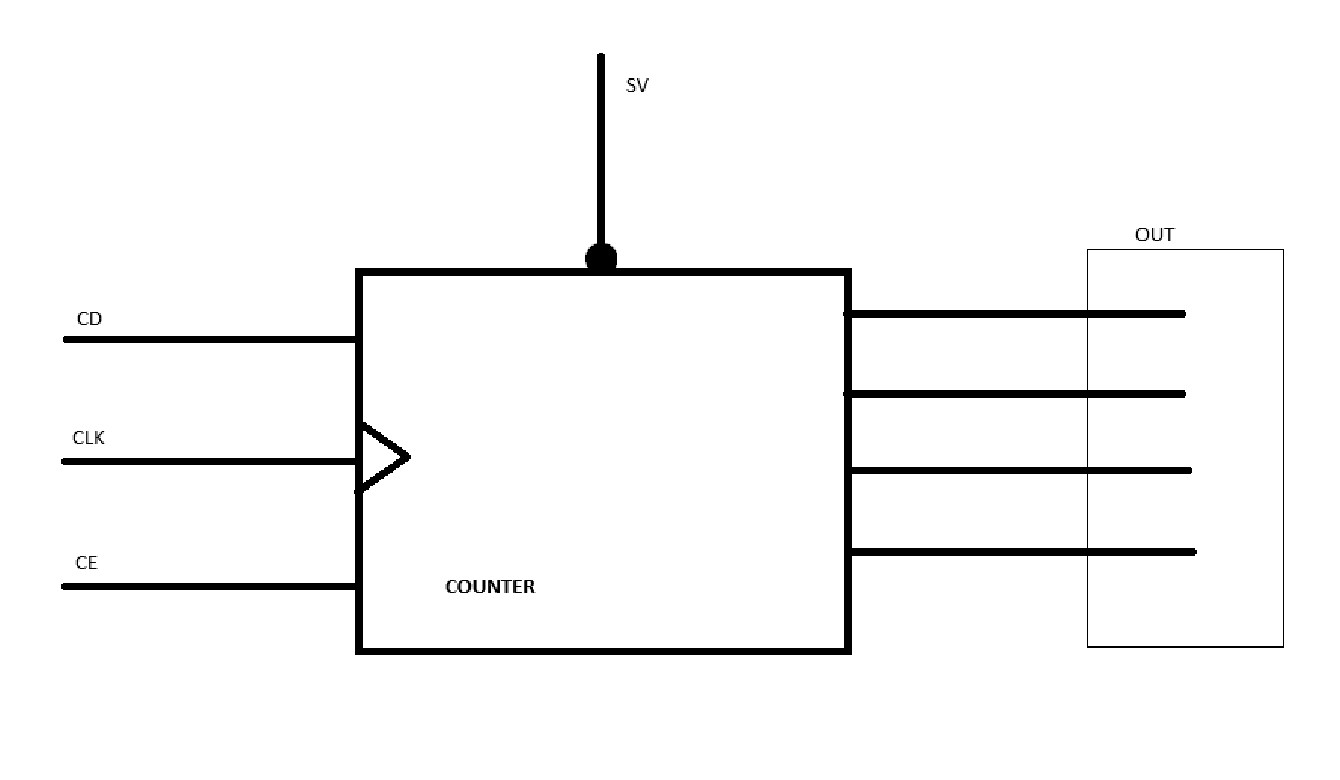
\includegraphics[height=10cm]{./images/Counter.jpg}
\end{figure}

\clearpage

\section{Kod Verilog}

\begin{lstlisting}

`timescale 1ns / 1ps


module main(
    input CLK,
	 input CE,
	 input CD,
	 input SV,
	 output [3:0] out
    );


reg [3:0] current_value;
reg [3:0] next_value;

initial
begin
	current_value = 4'b0000;
end


always @(posedge CLK or negedge SV)
begin
	if ( SV == 0) 
	begin
		if ( CD == 0 ) current_value = 4'b0000;
		else current_value = 4'b1111;
	end
	else if ( CE == 1 )	current_value = next_value;
end


always @ (current_value or CD)
begin
	if (CD == 0)
	begin
		case(current_value)
			4'b0000 : next_value = 4'b0001; //0 kod Aikena
			4'b0001 : next_value = 4'b0010; //1 
			4'b0010 : next_value = 4'b0011; //2
			4'b0011 : next_value = 4'b0100; //3
			4'b0100 : next_value = 4'b1011; //4
			4'b1011 : next_value = 4'b1100; //5
			4'b1100 : next_value = 4'b1101; //6
			4'b1101 : next_value = 4'b1110; //7
			4'b1110 : next_value = 4'b1111; //8
			4'b1111 : next_value = 4'b0000; //9
		endcase
	end
	else
	begin
		case(current_value)
			4'b0000 : next_value = 4'b1111; //0 kod Aikena
			4'b0001 : next_value = 4'b0000; //1 
			4'b0010 : next_value = 4'b0001; //2
			4'b0011 : next_value = 4'b0010; //3
			4'b0100 : next_value = 4'b0011; //4
			4'b1011 : next_value = 4'b0100; //5
			4'b1100 : next_value = 4'b1011; //6
			4'b1101 : next_value = 4'b1100; //7
			4'b1110 : next_value = 4'b1101; //8
			4'b1111 : next_value = 4'b1110; //9
		endcase
	end
end




assign out = current_value;

endmodule

\end{lstlisting}

\section{Kod w symulacji}

\begin{lstlisting}

	`timescale 1ns / 1ps

	module Sym1;
	
		// Inputs
		reg CLK;
		reg CE;
		reg CD;
		reg SV;
	
		// Outputs
		wire [3:0] out;
	
		// Instantiate the Unit Under Test (UUT)
		main uut (
			.CLK(CLK), 
			.CE(CE), 
			.CD(CD), 
			.SV(SV), 
			.out(out)
		);
		
		integer i;
		initial begin
			// Initialize Inputs
			CLK = 0;
			CE = 0;
			CD = 0;
			SV = 1;
	
			// Wait 100 ns for global reset to finish
			#50;
			
			//fork
			//begin
				CE = 1;
				for(i=0; i<11; i=i+1)
				begin
					#25 CLK = 1;
					#25 CLK = 0;
				end
			//end
				CE = 0;
				for(i=0; i<2; i=i+1)
				begin
					#25 CLK = 1;
					#25 CLK = 0;
				end
			
			#50;
			SV = 0;
			#50;
			SV = 1;
			//fork
			//begin
				CE = 1;
				for(i=0; i<11; i=i+1)
				begin
					#25 CLK = 1;
					#25 CLK = 0;
				end
			//end
				CE = 0;
				for(i=0; i<2; i=i+1)
				begin
					#25 CLK = 1;
					#25 CLK = 0;
				end
			
			CD = 1;
			
			#50;
			SV = 0;
			#50;
			SV = 1;
			
			CE = 1;
				for(i=0; i<11; i=i+1)
				begin
					#25 CLK = 1;
					#25 CLK = 0;
				end
			//end
				CE = 0;
				for(i=0; i<2; i=i+1)
				begin
					#25 CLK = 1;
					#25 CLK = 0;
				end
			
			#50;
			SV = 0;
			#50;
			SV = 1;
			//fork
			//begin
				CE = 1;
				for(i=0; i<11; i=i+1)
				begin
					#25 CLK = 1;
					#25 CLK = 0;
				end
			//end
				CE = 0;
				for(i=0; i<2; i=i+1)
				begin
					#25 CLK = 1;
					#25 CLK = 0;
				end
				
		end
	endmodule
	
	

\end{lstlisting}






\end{document}











% ================================================================
% ================================================================



% \begin{COPY}


% \begin{figure}[!htb]
%     \centering
%     \includegraphics[height=9cm]{./images/photo.png}
%     \caption{description here or leave blank or delete command}
%     \label{fig:1111}
% \end{figure}

% =====================================

% \begin{multicols}{2}
%     [
%     \section{First Section}
%     sdfsdfst esdfsdsf dsfsf 
%     ] 
%     sdfsdfsfsff dgfgd fgf dgfhfghgdf fghhf hg
% \end{multicols}

% =====================================

% \begin{minipage}{3cm}
%     Text sdfsf sdf sdf sdsfsdfsf ssdfdf sdsdff sdsdfsf sdsdff ssdfdf sdsdfsf sdf sdf sdsf  sfs
% \end{minipage}

% =====================================


% \begin{wrapfigure}{r}{0.5\textwidth}
%     \begin{center}
%       \includegraphics[width=0.48\textwidth]{./images/1.png}
%     \end{center}
%   \end{wrapfigure}

% =====================================


% \begin{figure}[!htb]
%     \begin{Large}
%         TYTUŁ WYKRESU
%     \end{Large}
%     \centering
%     \begin{tikzpicture}[]
    

%     \pgfplotsset{
%         ymin=-1e+2, ymax=1e+2,
%         xmin=-20, xmax=20,
%     }
    
%     \begin{axis}[
%         %enlargelimits=false,
%         height = 13cm,
%         width = 17.5cm,
%         xlabel = {x label $x$},
%         ylabel = {y label $f(x)$},
%         grid=major,
%      ]
    
%         \addplot [
%             mark size=3pt,
%             blue,
%             only marks,
%             point meta=explicit symbolic,
%             ] coordinates {
%                 (1, -20)
%                 (2, 0)
%                 (3, 20)
%             };

%         \addplot[
%             mark = none,
%             line width=1.7pt,
%             red,
%             /pgfplots/error bars/.cd,
%             ]
%             table [
%                 header=true,
%                 col sep=comma,
%                 ignore chars=\%,
%                 x=t,
%                 y=w,
%             ]{dir/csv.csv};
                    
%         \addplot [
%                 mark size=5pt,
%                 dashed,
%                 point meta=explicit symbolic,
%                 nodes near coords
%                 ] coordinates {
%                     (-3, 10400)
%                     (3, 10400)
%                 };
    
%         \addplot [
%                 mark size=5pt,
%                 green,
%                 line width=1.3pt,
%                 point meta=explicit symbolic,
%                 nodes near coords
%                 ] coordinates {
%                     (-100, 30)
%                     (100, 20)
%                 };

%         \addplot [
%             mark size=4pt,
%             mark=x,
%             solid,
%             line width=2pt,
%             black,
%             point meta=explicit symbolic,
%             nodes near coords
%             ] coordinates {
%                 (1, 10400)
%                 (10, 10400)
%             };

%         \node[] at (axis cs: 10, 10) {\Large $napis$};
    
%     \addlegendentry{legenda1}
%     \addlegendentry{legenda2}
%     \addlegendentry{legenda3}
%     \addlegendentry{legenda4}
% \end{axis}
% \end{tikzpicture}
% \end{figure}



% =====================================



% \begin{table}[!htb]
%     \setlength{\arrayrulewidth}{0.5mm}
%     \setlength{\tabcolsep}{20pt}
%     \renewcommand{\arraystretch}{1.7}
%     \begin{tabular}{ |p{5.5cm}|p{2.5cm}|  }
%     \hline
%     \multicolumn{2}{|c|}{0000000} \\
%     \hline
%     111 & 222 \\
%     \hline
%     $111$ & $222$ \\
%     \hline
%     \end{tabular}
% \end{table}
    


% =====================================



% \end{COPY}
